% Figure 1 -- MAGE algorithm flowchart
% Canvas 165 mm wide (= \textwidth of the manuscript, A4 with 2.25 cm margins).
% Insert at natural size:  \includegraphics{Figure1.pdf}   (scale 1:1)
% Text: Helvetica 7 pt (body), 6 pt (in-plot annotations), 8 pt bold panel labels;
% sub/superscripts >= 5 pt; Greek letters and all mathematical glyphs (operators,
% relations, delimiters, digits) from the Symbol font; Latin variables in Helvetica.
\documentclass[border=0pt]{standalone}
\usepackage[T1]{fontenc}
\usepackage{helvet}
\renewcommand{\familydefault}{\sfdefault}
\usepackage{amsmath,amssymb}
\usepackage[italic,symbolmax,symboldigits,mathaccents]{mathastext}
% remaining mathematical glyphs taken from the Symbol font as well
\DeclareSymbolFont{psysym}{U}{psy}{m}{n}
\DeclareMathSymbol{\rightarrow}{\mathrel}{psysym}{"AE}
\DeclareMathSymbol{\propto}{\mathrel}{psysym}{"B5}
\DeclareMathSymbol{\cdot}{\mathbin}{psysym}{"D7}
\DeclareMathSymbol{\symdots}{\mathinner}{psysym}{"BC}
\usepackage{bm}
\usepackage{tikz}
\usetikzlibrary{arrows.meta,calc,shapes.geometric}

\DeclareMathSizes{8}{8}{6}{5}
\DeclareMathSizes{7}{7}{5}{5}
\DeclareMathSizes{6}{6}{5}{5}

% colours (Wong palette based); colour is used for lines and fills only, text is black
\definecolor{colO}{HTML}{0072B2}
\definecolor{colN}{HTML}{009E73}
\definecolor{colA}{HTML}{CC79A7}
\definecolor{colB}{HTML}{E69F00}
\definecolor{colL}{HTML}{0072B2}
\definecolor{colV}{HTML}{D55E00}
\definecolor{bgO}{HTML}{EAF2F8}
\definecolor{bgN}{HTML}{E8F5F0}
\definecolor{bgA}{HTML}{F8EEF4}
\definecolor{bgB}{HTML}{FDF4E3}
\definecolor{bgG}{HTML}{F4F4F4}
\definecolor{arr}{HTML}{404040}

\newcommand{\fs}{\fontsize{7}{8.4}\selectfont}
\newcommand{\fsn}{\fontsize{6}{7.2}\selectfont}
\newcommand{\fsl}{\fontsize{8}{9.6}\selectfont\bfseries}
\newcommand{\veta}{\pmb{\eta}}
\newcommand{\vq}{\bm{q}}
\newcommand{\badge}[2]{\tikz[baseline=(bb.base)]\node[circle,fill=#1,text=black,inner sep=0pt,
  minimum size=3.4mm,font=\fontsize{5.5}{6}\selectfont\bfseries](bb){#2};}
\newcommand{\ttl}[3]{\badge{#1}{#2}\,\textbf{#3}}
\newcommand{\panel}[2]{{\fsl #1}\hspace{1.6mm}{\fs\bfseries #2}}

\begin{document}
\thickmuskip=4mu\medmuskip=3mu\thinmuskip=2.5mu
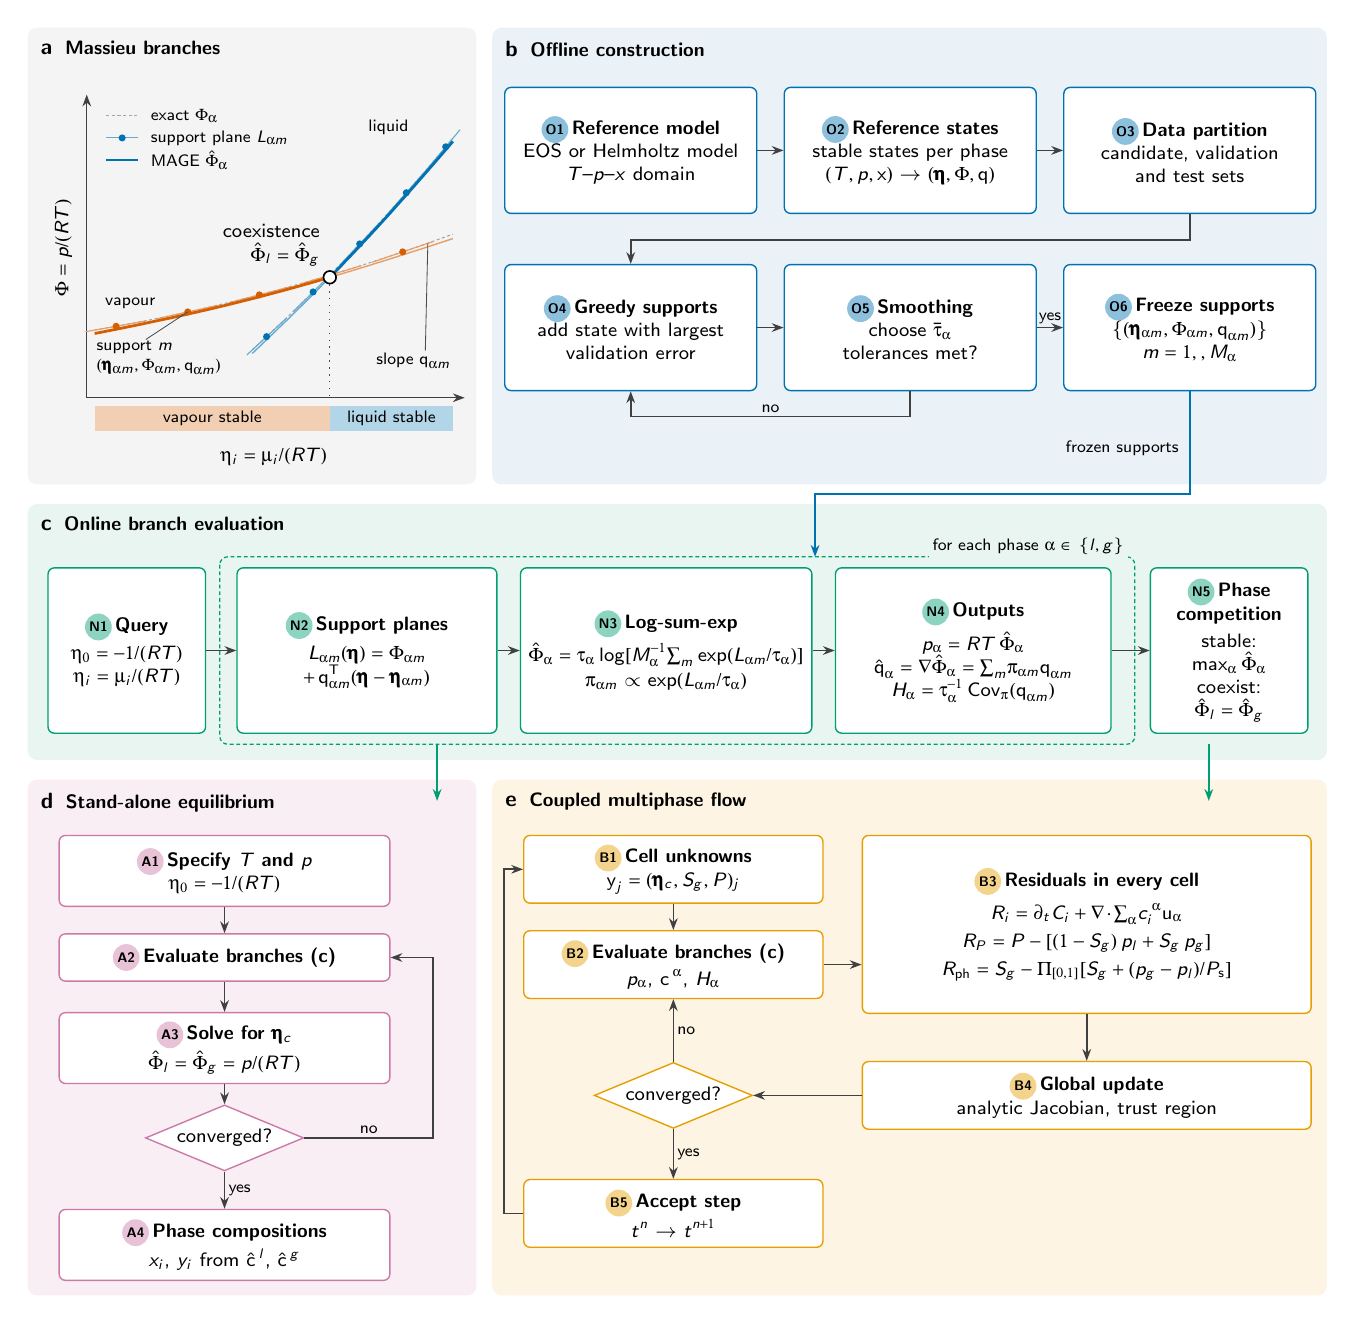
\begin{tikzpicture}[x=1mm,y=1mm,font=\fs,text=black,
  box/.style={draw=#1,line width=0.5pt,fill=white,rounded corners=0.8mm,
              align=flush center,inner sep=0.8mm},
  arrow/.style={-{Stealth[length=1.5mm,width=1.1mm]},line width=0.6pt,draw=arr},
  lab/.style={font=\fsn,inner sep=0.4mm},
  tanG/.style={colV!60,line width=0.4pt},
  tanL/.style={colL!60,line width=0.4pt},
  ob/.style={box=colO,text width=30.4mm,minimum height=16mm,anchor=north west},
  nb/.style={box=colN,minimum height=21mm,anchor=west},
  ab/.style={box=colA,text width=40.4mm,anchor=north},
  eb/.style={box=colB,text width=36.4mm,anchor=north}]

\path[use as bounding box] (0,0) rectangle (165,-161);

% ---------------- panel backgrounds ----------------
\fill[bgG,rounded corners=1.2mm] (0,0)      rectangle (57,-58);
\fill[bgO,rounded corners=1.2mm] (59,0)     rectangle (165,-58);
\fill[bgN,rounded corners=1.2mm] (0,-60.5)  rectangle (165,-93);
\fill[bgA,rounded corners=1.2mm] (0,-95.5)  rectangle (57,-161);
\fill[bgB,rounded corners=1.2mm] (59,-95.5) rectangle (165,-161);

% =====================================================================
% (a) finite-support Massieu branches
% =====================================================================
\node[anchor=north west,inner sep=0] at (1.6,-1.6) {\panel{a}{Massieu branches}};
\draw[arrow,line width=0.5pt] (7.5,-47) -- (7.5,-8.5);
\draw[arrow,line width=0.5pt] (7.5,-47) -- (55.5,-47);
\node[rotate=90,anchor=south] at (6.9,-28) {$\Phi=p/(RT)$};
\draw[gray!70,line width=0.4pt,dash pattern=on 1.1pt off 0.9pt] (8.50,-38.39) -- (8.88,-38.33) -- (9.26,-38.26) -- (9.64,-38.20) -- (10.02,-38.13) -- (10.40,-38.07) -- (10.78,-38.00) -- (11.15,-37.93) -- (11.53,-37.86) -- (11.91,-37.79) -- (12.29,-37.73) -- (12.67,-37.66) -- (13.05,-37.58) -- (13.43,-37.51) -- (13.81,-37.44) -- (14.19,-37.37) -- (14.57,-37.30) -- (14.95,-37.22) -- (15.32,-37.15) -- (15.70,-37.07) -- (16.08,-37.00) -- (16.46,-36.92) -- (16.84,-36.84) -- (17.22,-36.77) -- (17.60,-36.69) -- (17.98,-36.61) -- (18.36,-36.53) -- (18.74,-36.45) -- (19.12,-36.37) -- (19.50,-36.29) -- (19.88,-36.20) -- (20.25,-36.12) -- (20.63,-36.04) -- (21.01,-35.95) -- (21.39,-35.87) -- (21.77,-35.78) -- (22.15,-35.70) -- (22.53,-35.61) -- (22.91,-35.52) -- (23.29,-35.44) -- (23.67,-35.35) -- (24.05,-35.26) -- (24.42,-35.17) -- (24.80,-35.08) -- (25.18,-34.99) -- (25.56,-34.90) -- (25.94,-34.80) -- (26.32,-34.71) -- (26.70,-34.62) -- (27.08,-34.52) -- (27.46,-34.43) -- (27.84,-34.33) -- (28.22,-34.24) -- (28.60,-34.14) -- (28.98,-34.04) -- (29.35,-33.94) -- (29.73,-33.85) -- (30.11,-33.75) -- (30.49,-33.65) -- (30.87,-33.55) -- (31.25,-33.45) -- (31.63,-33.34) -- (32.01,-33.24) -- (32.39,-33.14) -- (32.77,-33.03) -- (33.15,-32.93) -- (33.53,-32.83) -- (33.90,-32.72) -- (34.28,-32.61) -- (34.66,-32.51) -- (35.04,-32.40) -- (35.42,-32.29) -- (35.80,-32.18) -- (36.18,-32.07) -- (36.56,-31.96) -- (36.94,-31.85) -- (37.32,-31.74) -- (37.70,-31.63) -- (38.08,-31.52) -- (38.45,-31.40) -- (38.83,-31.29) -- (39.21,-31.18) -- (39.59,-31.06) -- (39.97,-30.94) -- (40.35,-30.83) -- (40.73,-30.71) -- (41.11,-30.59) -- (41.49,-30.48) -- (41.87,-30.36) -- (42.25,-30.24) -- (42.62,-30.12) -- (43.00,-30.00) -- (43.38,-29.87) -- (43.76,-29.75) -- (44.14,-29.63) -- (44.52,-29.51) -- (44.90,-29.38) -- (45.28,-29.26) -- (45.66,-29.13) -- (46.04,-29.01) -- (46.42,-28.88) -- (46.80,-28.75) -- (47.17,-28.63) -- (47.55,-28.50) -- (47.93,-28.37) -- (48.31,-28.24) -- (48.69,-28.11) -- (49.07,-27.98) -- (49.45,-27.85) -- (49.83,-27.71) -- (50.21,-27.58) -- (50.59,-27.45) -- (50.97,-27.31) -- (51.35,-27.18) -- (51.73,-27.04) -- (52.10,-26.91) -- (52.48,-26.77) -- (52.86,-26.63) -- (53.24,-26.50) -- (53.62,-26.36) -- (54.00,-26.22);
\draw[gray!70,line width=0.4pt,dash pattern=on 1.1pt off 0.9pt] (28.52,-40.90) -- (28.84,-40.62) -- (29.16,-40.33) -- (29.48,-40.03) -- (29.79,-39.74) -- (30.11,-39.45) -- (30.43,-39.15) -- (30.75,-38.86) -- (31.07,-38.56) -- (31.39,-38.26) -- (31.71,-37.96) -- (32.02,-37.66) -- (32.34,-37.36) -- (32.66,-37.06) -- (32.98,-36.75) -- (33.30,-36.45) -- (33.62,-36.14) -- (33.93,-35.84) -- (34.25,-35.53) -- (34.57,-35.22) -- (34.89,-34.90) -- (35.21,-34.59) -- (35.53,-34.28) -- (35.85,-33.96) -- (36.16,-33.65) -- (36.48,-33.33) -- (36.80,-33.01) -- (37.12,-32.69) -- (37.44,-32.37) -- (37.76,-32.05) -- (38.08,-31.73) -- (38.39,-31.40) -- (38.71,-31.08) -- (39.03,-30.75) -- (39.35,-30.42) -- (39.67,-30.09) -- (39.99,-29.76) -- (40.30,-29.43) -- (40.62,-29.10) -- (40.94,-28.76) -- (41.26,-28.43) -- (41.58,-28.09) -- (41.90,-27.75) -- (42.22,-27.42) -- (42.53,-27.08) -- (42.85,-26.73) -- (43.17,-26.39) -- (43.49,-26.05) -- (43.81,-25.70) -- (44.13,-25.36) -- (44.45,-25.01) -- (44.76,-24.66) -- (45.08,-24.31) -- (45.40,-23.96) -- (45.72,-23.61) -- (46.04,-23.26) -- (46.36,-22.90) -- (46.67,-22.55) -- (46.99,-22.19) -- (47.31,-21.83) -- (47.63,-21.47) -- (47.95,-21.11) -- (48.27,-20.75) -- (48.59,-20.39) -- (48.90,-20.03) -- (49.22,-19.66) -- (49.54,-19.30) -- (49.86,-18.93) -- (50.18,-18.56) -- (50.50,-18.19) -- (50.82,-17.82) -- (51.13,-17.45) -- (51.45,-17.07) -- (51.77,-16.70) -- (52.09,-16.32) -- (52.41,-15.95) -- (52.73,-15.57) -- (53.04,-15.19) -- (53.36,-14.81) -- (53.68,-14.43) -- (54.00,-14.04);
\draw[tanG] (7.36,-38.61) -- (15.10,-37.23);
\draw[tanG] (16.46,-36.95) -- (24.20,-35.26);
\draw[tanG] (25.56,-34.93) -- (33.30,-32.92);
\draw[tanG] (34.66,-32.54) -- (42.40,-30.22);
\draw[tanG] (43.76,-29.79) -- (51.50,-27.16);
\draw[tanL] (27.84,-41.56) -- (32.84,-36.92);
\draw[tanL] (33.75,-36.05) -- (38.76,-31.07);
\draw[tanL] (39.67,-30.13) -- (44.67,-24.80);
\draw[tanL] (45.58,-23.80) -- (50.59,-18.12);
\draw[tanL] (50.59,-18.12) -- (54.91,-12.96);
\draw[colV!60,line width=0.5pt] (38.37,-31.70) -- (38.45,-31.68) -- (38.83,-31.57) -- (39.21,-31.45) -- (39.59,-31.34) -- (39.97,-31.23) -- (40.35,-31.11) -- (40.73,-31.00) -- (41.11,-30.89) -- (41.49,-30.77) -- (41.87,-30.65) -- (42.25,-30.54) -- (42.62,-30.42) -- (43.00,-30.31) -- (43.38,-30.19) -- (43.76,-30.07) -- (44.14,-29.95) -- (44.52,-29.84) -- (44.90,-29.72) -- (45.28,-29.60) -- (45.66,-29.48) -- (46.04,-29.36) -- (46.42,-29.24) -- (46.80,-29.12) -- (47.17,-29.00) -- (47.55,-28.88) -- (47.93,-28.76) -- (48.31,-28.64) -- (48.69,-28.51) -- (49.07,-28.39) -- (49.45,-28.27) -- (49.83,-28.15) -- (50.21,-28.03) -- (50.59,-27.90) -- (50.97,-27.78) -- (51.35,-27.66) -- (51.73,-27.53) -- (52.10,-27.41) -- (52.48,-27.29) -- (52.86,-27.16) -- (53.24,-27.04) -- (53.62,-26.91) -- (54.00,-26.79);
\draw[colL!60,line width=0.5pt] (28.52,-41.37) -- (28.84,-41.07) -- (29.16,-40.77) -- (29.48,-40.46) -- (29.79,-40.16) -- (30.11,-39.85) -- (30.43,-39.55) -- (30.75,-39.24) -- (31.07,-38.94) -- (31.39,-38.63) -- (31.71,-38.32) -- (32.02,-38.01) -- (32.34,-37.71) -- (32.66,-37.40) -- (32.98,-37.09) -- (33.30,-36.77) -- (33.62,-36.46) -- (33.93,-36.15) -- (34.25,-35.84) -- (34.57,-35.52) -- (34.89,-35.21) -- (35.21,-34.89) -- (35.53,-34.58) -- (35.85,-34.26) -- (36.16,-33.94) -- (36.48,-33.62) -- (36.80,-33.30) -- (37.12,-32.98) -- (37.44,-32.65) -- (37.76,-32.33) -- (38.08,-32.01) -- (38.37,-31.70);
\draw[colV,line width=1pt] (8.50,-38.84) -- (8.88,-38.77) -- (9.26,-38.69) -- (9.64,-38.62) -- (10.02,-38.54) -- (10.40,-38.47) -- (10.78,-38.39) -- (11.15,-38.32) -- (11.53,-38.24) -- (11.91,-38.16) -- (12.29,-38.09) -- (12.67,-38.01) -- (13.05,-37.93) -- (13.43,-37.86) -- (13.81,-37.78) -- (14.19,-37.70) -- (14.57,-37.62) -- (14.95,-37.54) -- (15.32,-37.46) -- (15.70,-37.38) -- (16.08,-37.30) -- (16.46,-37.22) -- (16.84,-37.14) -- (17.22,-37.06) -- (17.60,-36.98) -- (17.98,-36.90) -- (18.36,-36.82) -- (18.74,-36.73) -- (19.12,-36.65) -- (19.50,-36.56) -- (19.88,-36.48) -- (20.25,-36.40) -- (20.63,-36.31) -- (21.01,-36.22) -- (21.39,-36.14) -- (21.77,-36.05) -- (22.15,-35.96) -- (22.53,-35.88) -- (22.91,-35.79) -- (23.29,-35.70) -- (23.67,-35.61) -- (24.05,-35.52) -- (24.42,-35.43) -- (24.80,-35.34) -- (25.18,-35.25) -- (25.56,-35.15) -- (25.94,-35.06) -- (26.32,-34.97) -- (26.70,-34.87) -- (27.08,-34.78) -- (27.46,-34.68) -- (27.84,-34.59) -- (28.22,-34.49) -- (28.60,-34.40) -- (28.98,-34.30) -- (29.35,-34.20) -- (29.73,-34.10) -- (30.11,-34.00) -- (30.49,-33.90) -- (30.87,-33.80) -- (31.25,-33.70) -- (31.63,-33.60) -- (32.01,-33.50) -- (32.39,-33.40) -- (32.77,-33.29) -- (33.15,-33.19) -- (33.53,-33.08) -- (33.90,-32.98) -- (34.28,-32.87) -- (34.66,-32.77) -- (35.04,-32.66) -- (35.42,-32.55) -- (35.80,-32.45) -- (36.18,-32.34) -- (36.56,-32.23) -- (36.94,-32.12) -- (37.32,-32.01) -- (37.70,-31.90) -- (38.08,-31.79) -- (38.37,-31.70);
\draw[colL,line width=1pt] (38.37,-31.70) -- (38.39,-31.68) -- (38.71,-31.35) -- (39.03,-31.03) -- (39.35,-30.70) -- (39.67,-30.37) -- (39.99,-30.04) -- (40.30,-29.70) -- (40.62,-29.37) -- (40.94,-29.04) -- (41.26,-28.70) -- (41.58,-28.36) -- (41.90,-28.02) -- (42.22,-27.68) -- (42.53,-27.34) -- (42.85,-27.00) -- (43.17,-26.66) -- (43.49,-26.32) -- (43.81,-25.97) -- (44.13,-25.63) -- (44.45,-25.28) -- (44.76,-24.93) -- (45.08,-24.58) -- (45.40,-24.23) -- (45.72,-23.88) -- (46.04,-23.53) -- (46.36,-23.17) -- (46.67,-22.82) -- (46.99,-22.46) -- (47.31,-22.10) -- (47.63,-21.75) -- (47.95,-21.39) -- (48.27,-21.03) -- (48.59,-20.67) -- (48.90,-20.31) -- (49.22,-19.95) -- (49.54,-19.59) -- (49.86,-19.22) -- (50.18,-18.86) -- (50.50,-18.49) -- (50.82,-18.13) -- (51.13,-17.76) -- (51.45,-17.40) -- (51.77,-17.03) -- (52.09,-16.66) -- (52.41,-16.29) -- (52.73,-15.92) -- (53.04,-15.56) -- (53.36,-15.19) -- (53.68,-14.82) -- (54.00,-14.44);
\fill[colV] (11.23,-37.92) circle (0.45);
\fill[colV] (20.33,-36.10) circle (0.45);
\fill[colV] (29.43,-33.93) circle (0.45);
\fill[colV] (38.53,-31.38) circle (0.45);
\fill[colV] (47.63,-28.47) circle (0.45);
\fill[colL] (30.34,-39.24) circle (0.45);
\fill[colL] (36.25,-33.56) circle (0.45);
\fill[colL] (42.17,-27.46) circle (0.45);
\fill[colL] (48.09,-20.96) circle (0.45);
\fill[colL] (53.09,-15.13) circle (0.45);
\draw[black!70,dotted,line width=0.5pt] (38.37,-31.70) -- (38.37,-47);
\draw[fill=white,draw=black,line width=0.6pt] (38.37,-31.70) circle (0.8);
\node[anchor=south east,align=flush right,inner sep=0.4mm] at ($(38.37,-31.70)+(-0.8,0.9)$)
  {coexistence\\ $\hat\Phi_l=\hat\Phi_g$};
\node[anchor=south west,font=\fsn] at (8.6,-36.9) {vapour};
\node[anchor=east,font=\fsn] at (49.6,-12.6) {liquid};
\draw[black!70,line width=0.3pt] (20.33,-36.10) -- (15.0,-39.6);
\node[anchor=north west,align=flush left,font=\fsn,inner sep=0.3mm] at (8.4,-39.4)
  {support $m$\\ $(\veta_{\alpha m},\Phi_{\alpha m},\vq_{\alpha m})$};
\draw[black!70,line width=0.3pt] (50.82,-27.39) -- (50.5,-41.0);
\node[anchor=north,font=\fsn,inner sep=0.3mm] at (49.0,-40.9) {slope $\vq_{\alpha m}$};
% legend
\begin{scope}[shift={(10,-11.2)}]
  \draw[gray!70,line width=0.4pt,dash pattern=on 1.1pt off 0.9pt] (0,0) -- (4,0);
  \node[anchor=west,font=\fsn] at (4.4,0) {exact $\Phi_\alpha$};
  \draw[colL!60,line width=0.4pt] (0,-2.8) -- (4,-2.8); \fill[colL] (2,-2.8) circle (0.45);
  \node[anchor=west,font=\fsn] at (4.4,-2.8) {support plane $L_{\alpha m}$};
  \draw[colL,line width=1pt] (0,-5.6) -- (4,-5.6);
  \node[anchor=west,font=\fsn] at (4.4,-5.6) {MAGE $\hat\Phi_\alpha$};
\end{scope}
% stability bar (black text on light fills)
\fill[colV!30] (8.5,-48.0) rectangle (38.37,-51.2);
\fill[colL!30] (38.37,-48.0) rectangle (54,-51.2);
\node[font=\fsn] at ($(8.5,-49.6)!0.5!(38.37,-49.6)$) {vapour stable};
\node[font=\fsn] at ($(38.37,-49.6)!0.5!(54,-49.6)$) {liquid stable};
\node[anchor=north] at (31.25,-52.2) {$\eta_i=\mu_i/(RT)$};

% =====================================================================
% (b) offline construction
% =====================================================================
\node[anchor=north west,inner sep=0] at (60.6,-1.6) {\panel{b}{Offline construction}};
\node[ob] (O1) at (60.5,-7.5)  {\ttl{colO!45}{O1}{Reference model}\\ EOS or Helmholtz model\\ $T$--$p$--$x$ domain};
\node[ob] (O2) at (96.0,-7.5)  {\ttl{colO!45}{O2}{Reference states}\\ stable states per phase\\ $(T,p,\bm x)\rightarrow(\veta,\Phi,\vq)$};
\node[ob] (O3) at (131.5,-7.5) {\ttl{colO!45}{O3}{Data partition}\\ candidate, validation\\ and test sets};
\node[ob] (O4) at (60.5,-30.0) {\ttl{colO!45}{O4}{Greedy supports}\\ add state with largest\\ validation error};
\node[ob] (O5) at (96.0,-30.0) {\ttl{colO!45}{O5}{Smoothing}\\ choose $\bar\tau_\alpha$\\ tolerances met?};
\node[ob] (O6) at (131.5,-30.0){\ttl{colO!45}{O6}{Freeze supports}\\ $\{(\veta_{\alpha m},\Phi_{\alpha m},\vq_{\alpha m})\}$\\ $m=1,\symdots,M_\alpha$};
\draw[arrow] (O1.east) -- (O1.east -| O2.west);
\draw[arrow] (O2.east) -- (O2.east -| O3.west);
\draw[arrow] (O3.south) -- ++(0,-3.25) -| (O4.north);
\draw[arrow] (O4.east) -- (O4.east -| O5.west);
\draw[arrow] (O5.east) -- node[lab,above] {yes} (O5.east -| O6.west);
\draw[arrow] (O5.south) -- ++(0,-3.2) -| node[lab,pos=0.25,above] {no} (O4.south);

% link (b) -> (c): frozen supports feed the online kernel
\draw[arrow,line width=0.8pt,draw=colO] (O6.south) -- (O6.south |- 0,-59.25) -| (100,-67.2);
\node[anchor=east,font=\fsn] at (147.4,-53.4) {frozen supports};

% =====================================================================
% (c) online evaluation of a phase branch
% =====================================================================
\node[anchor=north west,inner sep=0] at (1.6,-62.1) {\panel{c}{Online branch evaluation}};
\draw[colN,line width=0.45pt,dash pattern=on 1.4pt off 1pt,rounded corners=1mm] (24.4,-67.2) rectangle (140.6,-91.0);
\node[anchor=south east,font=\fsn,fill=bgN,inner sep=0.5mm] at (139.8,-67.5) {for each phase $\alpha\in\{l,g\}$};
\node[nb,text width=18.4mm] (N1) at (2.5,-79.1)
  {\ttl{colN!45}{N1}{Query}\\[0.6mm] $\eta_0=-1/(RT)$\\ $\eta_i=\mu_i/(RT)$};
\node[nb,text width=31.4mm] (N2) at (26.5,-79.1)
  {\ttl{colN!45}{N2}{Support planes}\\[0.8mm] $L_{\alpha m}(\veta)=\Phi_{\alpha m}$\\ $+\,\vq_{\alpha m}^{\mathrm T}(\veta-\veta_{\alpha m})$};
\node[nb,text width=35.4mm] (N3) at (62.5,-79.1)
  {\ttl{colN!45}{N3}{Log-sum-exp}\\[0.4mm] $\hat\Phi_\alpha=\tau_\alpha\log[M_\alpha^{-1}{\textstyle\sum_m}\exp(L_{\alpha m}/\tau_\alpha)]$\\[0.3mm] $\pi_{\alpha m}\propto\exp(L_{\alpha m}/\tau_\alpha)$};
\node[nb,text width=33.4mm] (N4) at (102.5,-79.1)
  {\ttl{colN!45}{N4}{Outputs}\\[0.5mm] $p_\alpha=RT\,\hat\Phi_\alpha$\\ $\hat{\vq}_\alpha=\nabla\hat\Phi_\alpha={\textstyle\sum_m}\pi_{\alpha m}\vq_{\alpha m}$\\ $H_\alpha=\tau_\alpha^{-1}\,\mathrm{Cov}_{\pi}(\vq_{\alpha m})$};
\node[nb,text width=18.4mm] (N5) at (142.5,-79.1)
  {\ttl{colN!45}{N5}{Phase}\\ \textbf{competition}\\[0.5mm] stable:\\ $\max_\alpha\hat\Phi_\alpha$\\ coexist:\\ $\hat\Phi_l=\hat\Phi_g$};
\draw[arrow] (N1.east) -- (N2.west);
\draw[arrow] (N2.east) -- (N3.west);
\draw[arrow] (N3.east) -- (N4.west);
\draw[arrow] (N4.east) -- (N5.west);

% links (c) -> (d), (c) -> (e)
\draw[arrow,line width=0.8pt,draw=colN] (52,-91.0) -- (52,-98.2);
\draw[arrow,line width=0.8pt,draw=colN] (150,-91.0) -- (150,-98.2);

% =====================================================================
% (d) stand-alone phase equilibrium
% =====================================================================
\node[anchor=north west,inner sep=0] at (1.6,-97.1) {\panel{d}{Stand-alone equilibrium}};
\coordinate (xA) at (25,0);
\node[ab,minimum height=9mm] (A1) at (25,-102.5) {\ttl{colA!45}{A1}{Specify $T$ and $p$}\\ $\eta_0=-1/(RT)$};
\node[ab,minimum height=6mm] (A2) at (25,-115.0) {\ttl{colA!45}{A2}{Evaluate branches (c)}};
\node[ab,minimum height=9mm] (A3) at (25,-125.0) {\ttl{colA!45}{A3}{Solve for $\veta_c$}\\ $\hat\Phi_l=\hat\Phi_g=p/(RT)$};
\node[ab,minimum height=9mm] (A4) at (25,-150.0) {\ttl{colA!45}{A4}{Phase compositions}\\ $x_i$, $y_i$ from $\hat{\bm c}^{\,l}$, $\hat{\bm c}^{\,g}$};
\node[diamond,draw=colA,line width=0.5pt,fill=white,aspect=2.4,inner sep=0.4mm] (DA) at (25,-141.0) {converged?};
\draw[arrow] (A1.south) -- (A2.north);
\draw[arrow] (A2.south) -- (A3.north);
\draw[arrow] (A3.south) -- (DA.north);
\draw[arrow] (DA.south) -- node[lab,right] {yes} (A4.north);
\draw[arrow] (DA.east) -- node[lab,above] {no} (DA.east -| 51.5,0) |- (A2.east);

% =====================================================================
% (e) fully coupled multiphase flow
% =====================================================================
\node[anchor=north west,inner sep=0] at (60.6,-97.1) {\panel{e}{Coupled multiphase flow}};
% left column centred at x = 82, right column centred at x = 134.5
\node[eb,minimum height=8.6mm] (B1) at (82,-102.5) {\ttl{colB!45}{B1}{Cell unknowns}\\ $\bm y_j=(\veta_c,S_g,P)_j$};
\node[eb,minimum height=8.6mm] (B2) at (82,-114.6) {\ttl{colB!45}{B2}{Evaluate branches (c)}\\ $p_\alpha$, $\bm c^{\,\alpha}$, $H_\alpha$};
\node[eb,minimum height=8.6mm] (B5) at (82,-146.2) {\ttl{colB!45}{B5}{Accept step}\\ $t^n\rightarrow t^{n+1}$};
\node[box=colB,text width=55.4mm,minimum height=22.6mm,anchor=north] (B3) at (134.5,-102.5)
  {\ttl{colB!45}{B3}{Residuals in every cell}\\[0.8mm]
   $R_i=\partial_t C_i+\nabla\!\cdot\!{\textstyle\sum_\alpha} c_i^{\,\alpha}\bm u_\alpha$\\[0.6mm]
   $R_P=P-[(1-S_g)\,p_l+S_g\,p_g]$\\[0.6mm]
   $R_{\mathrm{ph}}=S_g-\Pi_{[0,1]}[S_g+(p_g-p_l)/P_{\mathrm{s}}]$};
\node[diamond,draw=colB,line width=0.5pt,fill=white,aspect=2.4,inner sep=0.4mm] (DB) at (82,-135.6) {converged?};
\node[box=colB,text width=55.4mm,minimum height=8.6mm,anchor=center] (B4) at (134.5,-135.6)
  {\ttl{colB!45}{B4}{Global update}\\ analytic Jacobian, trust region};
\draw[arrow] (B1.south) -- (B2.north);
\draw[arrow] (B2.east) -- (B2.east -| B3.west);
\draw[arrow] (B3.south) -- (B4.north);
\draw[arrow] (B4.west) -- (DB.east);
\draw[arrow] (DB.north) -- node[lab,right] {no} (B2.south);
\draw[arrow] (DB.south) -- node[lab,right] {yes} (B5.north);
\draw[arrow] (B5.west) -- ++(-2.4,0) |- (B1.west);

\end{tikzpicture}
\end{document}
